\documentclass[11pt,a4paper]{article}
%%%%%%%%%%%%%%%%%%%%%%%%%%%%%%%%%%%%%%%%%%%%%%%%%%%%%%%%
%                      PACKAGES                        %
%%%%%%%%%%%%%%%%%%%%%%%%%%%%%%%%%%%%%%%%%%%%%%%%%%%%%%%%

\usepackage[utf8]{inputenc}
\usepackage{graphicx} % Allows you to insert figures
\usepackage[export]{adjustbox}
\usepackage{booktabs}
\usepackage{amsmath} % Allows you to do equations
\usepackage{helvet}
\usepackage{hyperref}
\renewcommand{\familydefault}{\sfdefault}
\usepackage[a4paper, total={6.5in, 9.5in}]{geometry} % Formats the paper size, orientation, and margins
\linespread{1.1} % about 1.5 spacing in Word
\setlength{\parindent}{0pt} % no paragraph indents
\setlength{\parskip}{1em} % paragraphs separated by one line
\usepackage{listings}
\usepackage{enumitem}
\usepackage{xcolor}
\usepackage{hyperref}
\usepackage{pmboxdraw}
\usepackage{dirtree}

\hypersetup{
	colorlinks=true,
	urlcolor=cyan,
	linktoc=none,
}
\usepackage{fancyhdr}
\usepackage{float}

\pagestyle{fancy}
\fancyhead[L,C,R]{}
\fancyfoot[L]{Blix - AI Photo Editor}
\fancyfoot[C]{}
\fancyfoot[R]{\textbf{\thepage}}
\renewcommand{\headrulewidth}{0pt}
\renewcommand{\footrulewidth}{0.5pt}

\definecolor{codegreen}{rgb}{0,0.6,0}
\definecolor{codegray}{rgb}{0.5,0.5,0.5}
\definecolor{codepurple}{rgb}{0.58,0,0.82}
\definecolor{backcolour}{rgb}{0.95,0.95,0.92}

\usepackage{listings}

% Define TypeScript language style
\lstdefinelanguage{TypeScript}{
  keywords=[1]{class, constructor, let},
  keywordstyle=[1]\bfseries,
  keywords=[2]{string},
  keywordstyle=[2]\color{blue},
  sensitive=true,
  morestring=[b]',
  morestring=[b]"
}


\lstdefinestyle{mystyle}{
backgroundcolor=\color{backcolour},
commentstyle=\color{codegreen},
keywordstyle=\color{magenta},
numberstyle=\tiny\color{codegray},
stringstyle=\color{codepurple},
basicstyle=\ttfamily\footnotesize,
breakatwhitespace=false,
breaklines=true,
keepspaces=true,
numbers=left,
numbersep=5pt,
showspaces=false,
showstringspaces=false,
showtabs=false,
tabsize=2,
}

\lstset{style=mystyle}
\def\code#1{\texttt{#1}}

%%%%%%%%%%%%%%%%%%%%%%%%%%%%%%%%%%%%%%%%%%%%%%%%%%%%%%%%
%            TITLE PAGE & TABLE OF CONTENTS            %
%%%%%%%%%%%%%%%%%%%%%%%%%%%%%%%%%%%%%%%%%%%%%%%%%%%%%%%%

\begin{document}

\begin{titlepage}
	\centering
    % \includegraphics[width=0.5\textwidth]{your_logo.png}\par\vspace{1cm}
    {\scshape\LARGE Testing Policy Document\par}
    \vspace{1.5cm}
    {\huge\bfseries Blix - AI Photo Editor\par}
    \vspace{2.5cm}
    \begin{figure}[h]
        \centering % center the image
        \includegraphics[width=0.5\textwidth]{../pics/blix.png}
    \end{figure}
    \vspace{2.5cm}
    {\Large\itshape The Spanish Inquisition\par}

    \vfill
    {\large \today\par}
\end{titlepage}

\tableofcontents
\pagebreak

%%%%%%%%%%%%%%%%%%%%%%%%%%%%%%%%%%%%%%%%%%%%%%%%%%%%%%%%
%                MAIN DOCUMENT CONTENT                 %
%%%%%%%%%%%%%%%%%%%%%%%%%%%%%%%%%%%%%%%%%%%%%%%%%%%%%%%%

\addcontentsline{toc}{section}{Introduction}
\section*{Introduction}

Introducing Blix: An Advanced AI Photo Editor

Welcome to Blix, an innovative and sophisticated AI-powered photo editing
application. Blix sets itself apart by providing users with a seamless editing
experience through a powerful and intuitive interface, reminiscent of a digital
blender. This user manual will guide you through the features and
functionalities of Blix, enabling you to harness the full potential of this
cutting-edge editing tool.

Blix caters to users of all levels, from amateur photographers to seasoned
professionals, by streamlining the editing process and eliminating the need for
extensive knowledge of complex editing software. By presenting a visual
graph-based interface, akin to a blender, Blix enables effortless mixing and
matching of diverse editing effects.

As a user, you gain access to a vast array of editing possibilities. Whether you
wish to apply filters, fine-tune brightness and contrast, or add artistic
effects such as vignettes or vintage tones, Blix provides an extensive selection
of editing options. Each editing choice is represented as a node within the
graph, allowing for seamless connectivity and the creation of custom editing
flows tailored to your preferences.

What truly sets Blix apart is its integration of cutting-edge AI technology.
Through Blix, you can engage with an AI assistant that enhances your editing
journey. By sending prompts to the AI, you unlock a world of possibilities. The
AI assistant can recommend specific edits, suggest optimal adjustments, or even
manipulate the graph on your behalf, all based on your unique preferences and
the desired outcome.

In summary, Blix is an advanced AI photo editor that empowers users to elevate
their photography with ease and finesse. Its intuitive graph-based interface,
extensive editing options, and integration with an AI assistant create a
harmonious environment for realizing your creative vision. This user manual will
serve as your comprehensive guide, enabling you to navigate the features of Blix
and unlock the full potential of your photo editing capabilities.

\pagebreak


\addcontentsline{toc}{section}{General Testing Characteristics}
\section*{General Testing Characteristics}   

During the continued developement of Blix, we have made use of a variety of
testing techniques. These techniques include unit testing, integration testing,
and end to end testing. In order to facilitate the testing process, we have made
use of a variety of tools. These tools include Jest, playwright, codecov and
github workflows. These tools have been used to test the functionality of the
application, automate the testing process, and ensure that the application is
properly covered by tests.


\addcontentsline{toc}{subsection}{Unit Testing}
\subsection*{Unit Testing}

Unit testing is a software testing method by which individual units of source
code are tested to determine whether they are working as intended. Blix has been
extensively tested using unit testing. This has been done using the Jest
framework. 

Jest is a JavaScript testing framework designed to ensure correctness of any
JavaScript/Typescript codebase. All of the core functionality of Blix has been
unit tested. This includes the functionality of the graph, the AI assistant, the
plugins, and the user interface, ensuring that each function executes correctly
at an atomic level in isolation. 

\addcontentsline{toc}{subsection}{Integration Testing}
\subsection*{Integration Testing}

Integration testing is the phase in software testing in which individual
software modules are combined and tested as a group. In the various subsystems
of Blix, integration tests have been used to ensure that the subsystems are
working together as intended. This has also been done using the Jest framework.
Each subsystem in their entirety as well as the subsystems communicating with
each other have been tested, ensuring that all interactions between systems and
the travel of data between systems is correct.

Minimal or no mocking is used for Integration testing as we want to test the
actual functionality of the application such that communication and interaction
between systems is tested, and not the atomic operations of each system. Mocks
are mainly used for integration tests when testing a subsystem that uses an
external resource such as an api request. 


\subsubsection*{JEST}
\addcontentsline{toc}{subsubsection}{JEST}

The reason why we chose Jest for our unit and integration testing is because it
is a very popular testing framework that has TypeScript support and meshes
easily with the rollup of our electron app. Jest is easy to use and has a lot of
functionality that makes testing easier, such as mocking and code coverage.

Furthermore due to the popularity of Jest, there is a lot of documentation and
support for it, which makes it easy to use and learn, which was essential
considering our lack of experience with testing frameworks

\addcontentsline{toc}{subsection}{End to End Testing}
\subsection*{End to End Testing}

End-to-end testing is a technique used to test whether the flow of an
application is performing as designed from start to finish. The purpose of
carrying out end-to-end tests is to identify system dependencies and to ensure
that the right information is passed between various system components and
systems. Blix has multiple end to end tests that test the correct functionality
of the application as a whole. These tests are done using the playwright
framework. Playwright is a Node.js library to automate Chromium, Firefox and
WebKit with a single API. 

These end to end tests either start in the backend or the frontend, and ensure
that all the systems execute according to specification untill the request or
result finally reaches the other end of the stack. End to end testing is
inherently slow and all-encompasing, and therefore there are fewer tests for it.
These tests are done to ensure that the application is working as a whole, and
that all the systems are communicating correctly.


\subsubsection*{Playwright}

Playwright was chosen for the end-to-end tests due to its support for multiple
platforms such as Windows, Linux and MacOS and has built-in integrations to
interact with jest, our testing framework of choice for unit and integration
testing. 

Furthermore playwright is relatively easy to use and has a lot of documentation
and support, due to its popularity, which makes it easy to learn and use.

\addcontentsline{toc}{subsection}{CICD}
\subsection*{CICD}

For the purposes of testing, we have made use of github workflows. Github
workflows are a feature of github that allow for the automation of tasks. We
have made use of github workflows to automate the testing process. 

This is done by running the tests on every pull request, and on every push to
the main branch. This ensures that the application is always tested before any
changes are merged into the main branch.

The tests that are automated for this purpose consist of : 
\begin{itemize}
  \item Unit tests
  \item Integration tests
  \item End to end tests
  \item Building the application
  \item Linting the application
  \item Secret protection
  \item Code coverage
\end{itemize}

\begin{figure}[htbp]
  \centering
  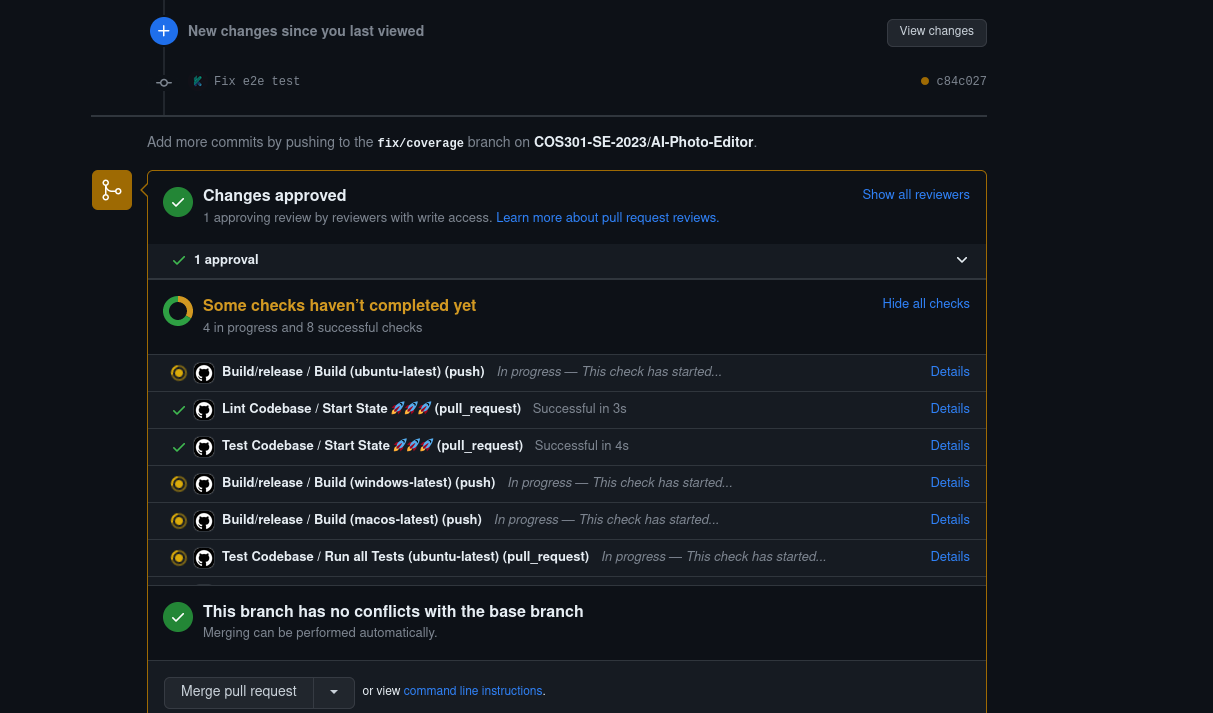
\includegraphics[width=0.95\textwidth]{../pics/cicd.png}
  \caption{Continuous Integration and Continuous Deployment (CI/CD) Pipeline}
\end{figure}

The reason why we chose github workflows for our cicd pipeline is because it
enables us to build and test our app for Windows,Linux and MacOS without having
to set up a local environment for each of these operating systems. This is done
by using the github hosted runners. These runners are virtual machines that run
the github workflows. 

The github hosted runners are free to use for open source projects, and
therefore we can use them for our project, allowing us to cut costs and save
time. Furthermore github workflows are easy to set up and use, and are
integrated with github, allowing us to easily automate our testing process.

For a more in depth view of our cicd pipeline, please refer to the following
link : \url{https://github.com/COS301-SE-2023/AI-Photo-Editor/actions}

\begin{figure}[H]
  \centering
  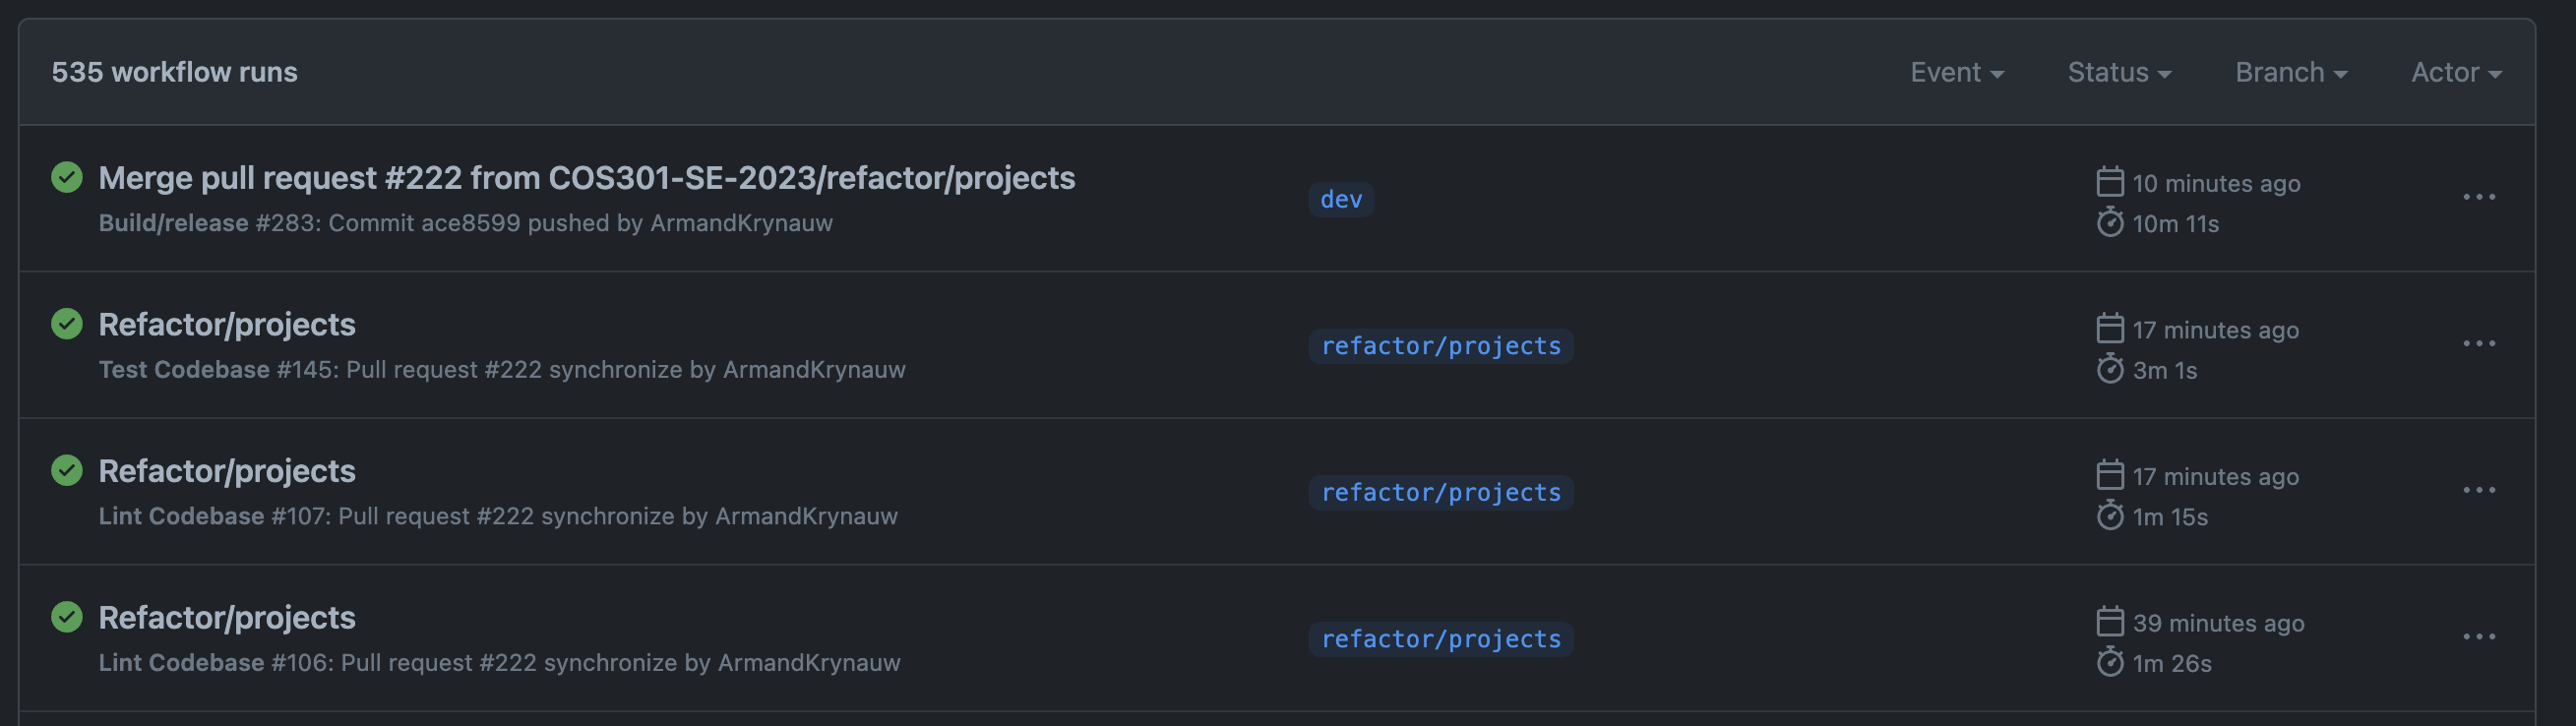
\includegraphics[width=0.95\textwidth]{../pics/actions.png}
  \caption{Github Actions}
\end{figure}

\pagebreak

\addcontentsline{toc}{section}{Software Quality Assurance}
\section*{Software Quality Assurance}

The software requirements specification outlines quality criteria that must be
assessed, measured, and validated for compliance within the project. These
criteria are summarized briefly here and elaborated upon in dedicated sections.

\addcontentsline{toc}{subsection}{Software Quality Assurance}

\begin{enumerate}[label*=\arabic*.]
  \item Customizability \& Extensibility
  \item Compatibility
  \item Performance
  \item Usability
  \item Security
\end{enumerate}

\addcontentsline{toc}{subsection}{Customizability \& Extensibility}
\subsection*{Customizability \& Extensibility}

Customizability and extensibility refer to the ability of an application to be
modified to meet different user needs and accommodate future enhancements. These
requirements are important to ensure the longevity and relevance of the software
in a rapidly changing technological environment.

Customizability enables users to adjust the software's functionalities based on
their individual preferences and requirements, improving user satisfaction and
productivity. Extensibility, on the other hand, ensures that our software is
ready for future expansion, allowing us to add new features and functionalities
without making major changes to the existing system structure.

The entirety of Blix was built from the ground-up to be as extensible as
possible. Blix has an extensive plugin system that allows for the easy addition
of new plugins that can enable a wide range of new features and workflows for
users.  

\subsubsection*{Quantification - Extensibility}

The system's extensibility has been designed specifically to support the
integration of both developer and user-generated plugins. The modular
architecture of the system minimizes the potential impact on the existing system
during the integration of new plugins.

To quantify extensibility, the system's performance was evaluated by integrating
several new plugins and modules. The test result was successful, with no
disruption to the existing functionalities. Currently, Blix accommodates a
single built-in plugin that showcases the capacity to present any form of media
or data flowing within the system. The primary functionality of the system is
augmented with six specific plugins designed to meet the system's requirements,
which include:

\begin{enumerate}
  \item A Mathematical Plugin enabling fundamental mathematical operations. 
  \item A Logic Plugin facilitating basic logical operations.
  \item A Basic Image Editing Plugin with one-way data binding from the graph to
  the media.
  \item An Advanced Image Editing Plugin facilitating two-way data binding from
  the graph to the media and vice-versa.
\end{enumerate}

It is noteworthy that the plugins were integrated seamlessly, and no
functionality was disrupted during their addition. This demonstrates the
system's high level of extensibility. The system's ability to readily adapt and
incorporate new plugins will continue to be a critical metric for measuring
extensibility in future developments.

\subsubsection*{Quantification - Customizability}

The system offers a high degree of customizability to users, providing an
adaptable interface that users can modify to suit their preferences. This
includes a fully customizable layout, allowing users to add, remove, and
rearrange the tiles integrated within the system. Additionally, plugin
developers have the freedom to customize and create their own unique tiles.

To further enhance customizability, the system allows users to create and save
custom graphs and workflows, providing flexibility to operate as per their
unique needs. Another essential feature is the ability to customize preferred
settings such as hotkeys, which are uniformly integrated throughout the system,
enhancing ease of use and efficiency.

Customizability has been quantitatively assessed through a combination of user
feedback and usability testing conducted throughout the development process. The
metrics derived from these assessments served as a benchmark for the system's
customizability and enabled continuous improvements to better cater to user
preferences and enhance overall user experience.

\addcontentsline{toc}{subsection}{Compatibility}
\subsection*{Compatibility}

Compatibility assesses the ability the application to operate effectively across
various platforms and systems. In today's diverse and interconnected digital
world, compatibility is an essential attribute that ensures our software can
reach and serve a broader user base, regardless of their chosen operating system
or device.

Our application is designed as a cross-platform desktop solution, capable of
running seamlessly on multiple operating systems such as Windows, macOS, and
Linux. This cross-platform compatibility enables us to provide a consistent user
experience and maintain the full functionality of our software across all
supported platforms.

\subsubsection*{Quantification}

Our application is designed with cross-platform compatibility in mind, offering
a unified user experience across all supported platforms. This compatibility
guarantees that updates or enhancements made to the system are simultaneously
available to all users, regardless of the platform they are using.

Market share analysis reveals that:

\begin{enumerate}
  \item Windows holds a 70\% market share
  \item MacOS comprises 20\% of the market
  \item Linux contributes to a 3\% market share
\end{enumerate}

Therefore, our focus on compatibility ensures we cater to a significant
proportion of the user market, particularly those utilizing Windows 10 and
Ubuntu. In addition, our application supports both ARM and x86 architectures,
thus facilitating its reach to a wider user base. This includes supporting users
of the new Apple Silicon machines.

The minimum system requirements for our application to function optimally across
these platforms are:

\begin{enumerate}
  \item Windows: 7/10 - Intel Quad Core i5 or AMD equivalent with 4GB RAM and
  2GB of free disk space.
  \item MacOS: 10.13 - Any new Mac with an Intel processor or Apple Silicon with
  4GB RAM and 2GB of free disk space.
  \item Ubuntu: 18.04 - Intel Quad Core i5 or AMD equivalent with 4GB RAM and
  2GB of free disk space.
\end{enumerate}

Our quantification of compatibility is not limited to design alone. We have
performed rigorous testing on all supported platforms throughout the development
process. This diligence ensures that our application delivers consistent
performance and user experience, regardless of the platform in use.

\addcontentsline{toc}{subsection}{Performance}
\subsection*{Performance}

\addcontentsline{toc}{subsection}{Usability}
\subsection*{Usability}


\addcontentsline{toc}{subsection}{Security}
\subsection*{Security}

Security focuses on safeguarding Blix, its data, and its users from potential
threats. In the digital era, where cyber threats are continually evolving, a
robust security approach is indispensable to maintain user trust and protect
valuable data.

\subsubsection*{Quantification}

Blix has been engineered with an emphasis on offline usage, providing user
convenience while additionally enhancing its security posture. However, our
commitment to security extends beyond this design consideration. We have
integrated several security measures and best practices aimed at achieving
optimal security standards. These include:

\textbf{Sandboxing of renderers and webviews}

A core security feature of our application is the sandboxing of renderers and
webviews. This mechanism isolates these components into a separate process. This
segregation restricts their capabilities and limits their access to sensitive
data or system resources, effectively thwarting potential security breaches.
This practice aligns with OWASP's recommendation of implementing secure
defaults.

\textbf{Context isolation}

We have further fortified our application's security by implementing context
isolation. This security measure delineates the Electron runtime's context from
the application's context, thereby shielding powerful internal Electron APIs
from malicious scripts. This practice is consistent with OWASP's principle of
least privilege.

\textbf{Disabling of Node integration in renderers}

To safeguard our application from remote code execution attacks, Node.js
integration within our renderers has been disabled. This strategy obstructs
malicious scripts from obtaining direct access to low-level system resources,
significantly enhancing overall security.

\textbf{Open-source Plugin code}

In our pursuit of transparency and collaborative security improvement, the code
for our plugins is open-source. This allows for community-driven security audits
and contributes to the overall hardening of our application's security.

In conclusion, these security measures - sandboxing, context isolation,
disabling of Node integration - along with our open-source plugin code, work in
tandem to create a robust security environment for our application. In alignment
with OWASP guidelines, these strategies ensure our application is resilient
against a plethora of security threats, thereby safeguarding our users and their
data.

\end{document}